\documentclass{article}
\usepackage[utf8]{inputenc}
\usepackage{graphicx}
\graphicspath{{Images/}}
\usepackage[export]{adjustbox}
\usepackage{amsmath}
\usepackage{hyperref}
\hypersetup{colorlinks=true,citecolor=yellow,linkcolor=blue,urlcolor=red}
\date{January 26,2022}
\pagebreak

\begin{document}

\tableofcontents
\pagebreak
\section{Dermatoscope}

A dermatoscope is a hand-held visual aid device a doctor or person can use to examine and diagnose skin lesions and diseases, such as melanoma. It can also help a person examine the scalp, hair, and nails.

\subsection{How does a dermatoscope work?}
\begin{figure} [h]
     \centering
     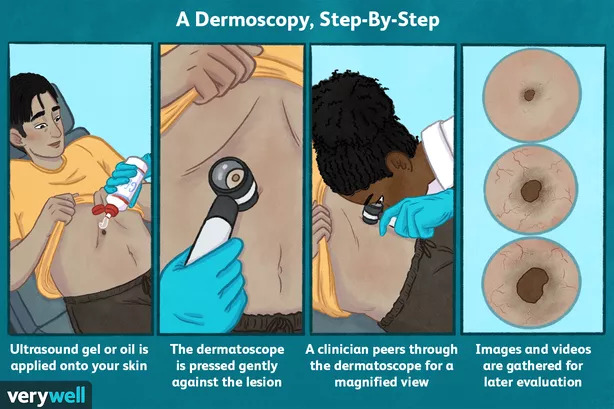
\includegraphics[scale=0.5]{Dermatoscope working.jpg}
     \caption{Dermatoscope working}
     \label{fig:dermatoscope working}
 \end{figure}
Dermatoscope features a light source and a magnifier and works a little like a magnifying glass.
\begin{itemize}
\item a traditional dermatoscope magnifies the view of the skin by 10 times. Video dermatoscopes can increase this to around 70–100 times.
\item The light on the dermatoscope helps illuminate the skin in a special way, allowing a doctor to examine lesions without the light bouncing off of dry or oily skin, which would make it more difficult to see.
\item Dermatoscopes can also take pictures as people use them. Doctors may examine these photos later.
\end{itemize}


\subsection{What can a dermatoscope see?}
A dermatoscope greatly magnifies the outer layers of the skin. Doctors can use them to look for colors, patterns, or shapes that can help distinguish and diagnose various skin conditions.
\subsection{Types of dermatoscopes}
\begin{figure} [h]
    \centering
    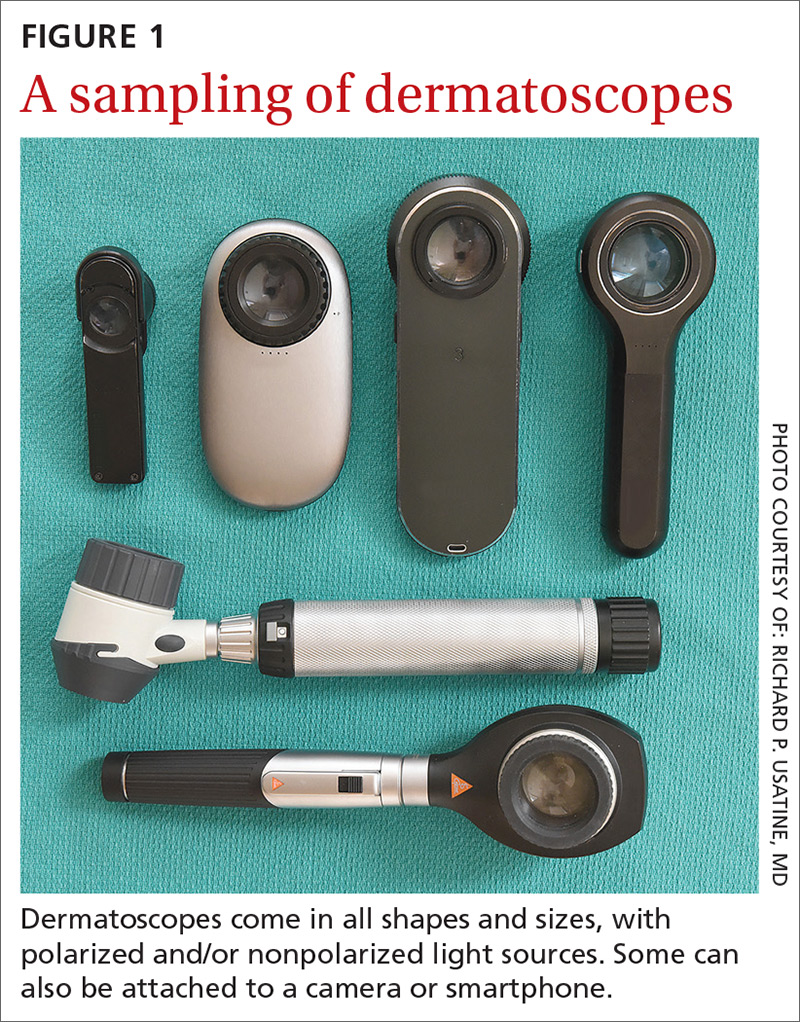
\includegraphics[scale=0.3]{Dermatoscopes.jpg}
    \caption{Different types of dermatoscopes}
    \label{fig_types of dermatoscopes}
\end{figure}
There are three main types of dermatoscopes. They include:
\begin{itemize}
\item \textbf{Hand-held dermatoscope}: This type of dermatoscope is a simple hand-held device with a built-in light. They can magnify images by about 10–20 times. They do not connect to a monitor.
\item \textbf{Dermatoscope connected to a camera}: These dermatoscopes allow photos to be taken of the skin for later examination.
\item \textbf{Dermatoscope connected to a viewing device}: This type of dermatoscope allows for pictures, video, and shared viewing with doctors and patients during the examination.
\end{itemize}
\subsection{Are dermatoscopes accurate?}
dermatoscopes are more accurate in diagnosing melanomas than the naked eye alone when utilized by a trained professional. This is crucial as it can save a person time and potentially prevent them from undergoing surgery unnecessarily.
\subsubsection{Factors that can affect accuracy}
Although dermatoscopes can give considerable benefits to a doctor as opposed to the naked eye, there are some factors that may affect their accuracy:
\begin{itemize}
\item Unclean skin
\item Darker skin tones
\item Differing types of dermatoscope: doctors may get varying results if they use different dermatoscopes to examine the skin.
\end{itemize}
\pagebreak
\section{Gamma Cameras}
Gamma cameras or scintillation cameras are pieces of apparatus which allow radiologists to carry out 'scintigraphy scans', tests which provide detailed diagnoses about the functioning of the thyroid, the heart, the lungs and many other parts of the body. Scintigraphy scans get their name from the ability of some crystals (such as sodium iodide) to scintillate (in other words, emit sparks) when exposed to radiation.

\begin{itemize}
\item The gamma camera or scintillation camera was invented by the American physicist H.O. Anger in Berkeley in 1957.
\end{itemize}
\begin{figure} [h]
    \centering
    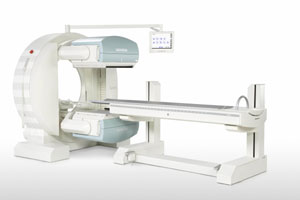
\includegraphics{siemens_300.jpg}
    \caption{Gamma camera}
    \label{fig:gamma camera}
\end{figure}
\subsection{How does a gamma camera work?}
\begin{itemize}
\item To begin with, a tracer or radiopharmaceutical is administered to the patient orally, intravenously or through inhalation. The patient’s body contains radioactive tracer for a brief period, during which gamma cameras can be used to generate images. 
\item These cameras image the radiation from the tracer, with Technetium-99m being the most commonly used tracer. It has a relatively long half-life of six hours and can be incorporated into a variety of molecules making it capable of targeting different systems of the body. As the tracer travels through the human body, it emits radiation that can be picked up and tracked by a crystal in the camera that sparks or scintillates (flashes) in response to exposure to gamma rays.
\item The crystal in the camera is positioned in front of an array of light sensors so that the flashes of light upon exposure get converted into an electrical signal. This is why the camera is also known as a scintillating camera. This technology helps to gauge functioning and health of various body structures and organs as experts can recognize conditions based on the accumulation or exclusion of tracer from certain areas.
\end{itemize}
 \begin{figure}
     \centering
     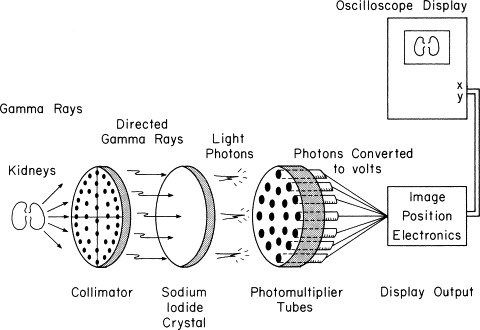
\includegraphics[scale=0.7]{ezgif.com-gif-maker(2).jpg}
     \caption{Gamma Camera Working}
     \label{fig:gamma camera working}
 \end{figure}
 
\subsection{What is a Gamma Camera used for?}
Gamma cameras are extremely important for radiologists as they enable them to perform what are medically called "Scintigraphy scans" that reveal detailed information about the functioning of various organs such as lungs, heart, thyroid, parathyroids, liver, kidneys and adrenals to name a few. This makes them extremely useful in medical care as they are used in the diagnosis of health conditions and also to monitor follow up treatment. They can also pick up spread of cancers to bones or organs and these appear as hot spots.

\subsection{How is Safety Ensured while using a Gamma Camera?}
Patients are exposed to some amount of radiation during such procedures, but the amount varies depending on the specific procedure, the organ or structure being examined and the physical dimensions of the patient. Either way, health care providers follow stringent safety practices and will only administer the lowest possible dosage that can provide high quality results, so as to minimize unnecessary exposure to the drug.

\subsection{Benefits and risks of a Gamma Camera scan}
\subsubsection{Benefits of the test}
\begin{itemize}
\item The scan can help in early detection of cancer.
\item he test can help in deciding if additional interventional procedures will provide any benefit or not.
\item Provides a low-cost and high-resolution imaging which can help avoid certain interventional procedures.
\end{itemize}

\subsubsection{Risks of test}
\begin{itemize}
\item Exposure to radiation: During a scintigraphy scan,  our body is briefly exposed to more radiation than you would be during a plain X-ray.
\item Harm to unborn babies (pregnant ladies)
\item Reactions to contrast material
\end{itemize}
\pagebreak

\section{High-performance liquid chromatography(HPLC)}

High Performance Liquid Chromatography (HPLC) is a form of column chromatography that pumps a sample mixture or analyte in a solvent (known as the mobile phase) at high pressure through a column with chromatographic packing material (stationary phase). The sample is carried by a moving carrier gas stream of helium or nitrogen. HPLC has the ability to separate, and identify compounds that are present in any sample that can be dissolved in a liquid in trace concentrations as low as parts per trillion. Because of this versatility, HPLC is used in a variety of industrial and scientific applications, such as pharmaceutical, environmental, forensics, and chemicals.
\begin{figure} [h]
    \centering
    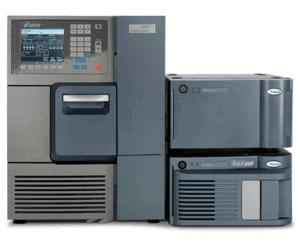
\includegraphics{HPLC-system.png}
    \caption{HPLC system}
    \label{fig:hplc system}
\end{figure}
\subsection{How HPLC Instrument works?}
\begin{itemize}
\item For chromatography to occur, there must be a stationary phase and a mobile phase. The adsorbent normally is a solid (or a liquid) in nature and the mobile-phase normally a liquid or a gaseous matter.
\item The solvent is responsible for carrying the constituents of the subject mixture through the stationary phase. More lagging is experienced in components which interact more with the stationary phase.
\item In HPLC, a pressure pump forces the solvent (mobile phase) together with the subject mixture through a column with the stationary phase material(normally a solid). In the column, each component of the mixture will interact differently with the stationary phase.
\item Due to the interaction with the stationary phase, these components in the mixture will separate, each exiting the column on its own. It is important that the temperature of both the phases be kept constant.
\end{itemize}
\begin{figure} [h]
    \centering
    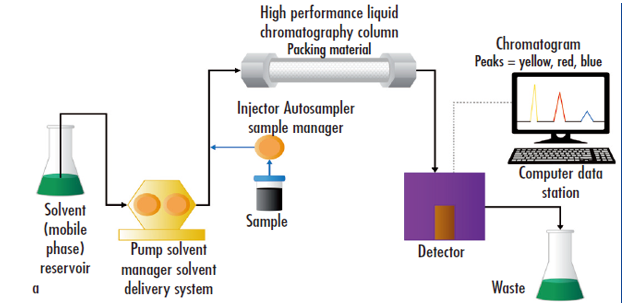
\includegraphics[scale=0.75,center]{high-performance-liquid-chromatography-service-1.png}
    \caption{HPLC System working}
    \label{fig:hplc system working}
\end{figure}
\subsubsection{Components of an HPLC Instrument}
\begin{itemize}
\item \textbf{Columns}: This is where the stationary-phase material is placed. It is about 5 mm in diameter and can be as long as 300m.
\item \textbf{Pumps}: These supply high pressure of up to 400 atms that forces the mixture and solvent through the column.
\item \textbf{Sampler Injector}: This delivers the mixture in the subject to the mobile phase.
\item \textbf{Detector}: This device is located at the and of the column. It facilitates quantitative analysis of the different components of the mixture. The device detects the components as they flow out of the column. UV-spectroscopy is a commonly used detector
\end{itemize}
\subsection{Different Types Of High Performance Liquid Chromatography}
\begin{itemize}
\item  \textbf{Size-exclusion HPLC}:The material used in the stationary phase in this type operates on the basis of components' molecular size.
\item \textbf{Ion-exchange HPLC}: This type of HPLC operates on the basis of ionic charges. The adsorbent has ionic charges that are opposite to the subject constituents' ionic charges.
\item \textbf{Normal phase HPLC}: The basis for the operation of normal phase HPLC is polarity. The solvent is non-polar (normally an organic compound) and adsorbent polar.
\item \textbf{Reverse Phase HPLC}: in this type, the solvent polar (hydrophilic) and adsorbent non-polar. It is the opposite of the normal phase HPLC. The nonpolar components will take longer to exit the column.
\end{itemize}
\subsection{Uses Of HPLC In Pharmaceuticals}
HPLC is generally used in pharmaceutical industry, as it can provide the precise results that are required. The results can be used to analyse finished drug products and their ingredients quantitatively and qualitatively during the manufacturing process.
\begin{figure} [h]
    \centering
    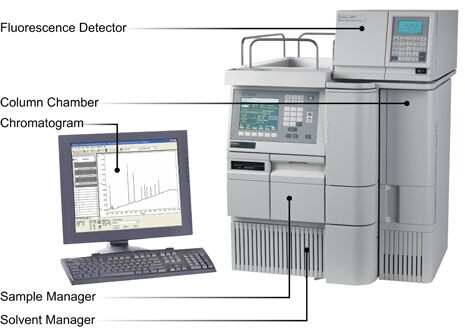
\includegraphics[scale=0.7]{primer_F_AllianceHPLCSystem.jpg}
    \caption{A Typical HPLC System}
    \label{fig:a typical hplc system}
\end{figure}
\pagebreak

\section{Keratometer}
A keratometer, also known as an ophthalmometer, is a diagnostic instrument for measuring the curvature of the anterior surface of the cornea, particularly for assessing the extent and axis of astigmatism.
\begin{figure} [h]
    \centering
    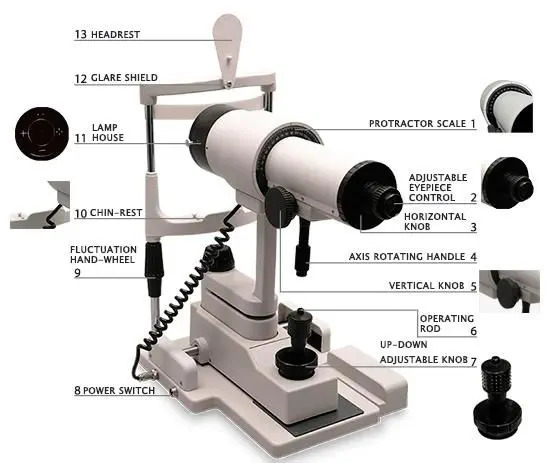
\includegraphics[scale=0.7,center]{ezgif.com-gif-maker (1).jpg}
    \caption{Keratometer}
    \label{fig:keratometer}
\end{figure}
\subsection{Working of Keratometer}
\begin{itemize}
\item This device measures the curvature of the anterior corneal surface based on the power of a reflecting surface. It does this by measuring the size of an image reflected from 2 paracentral points and utilizes doubling prisms to stabilize the image enabling more accurate focusing.
\item Principle of keratometer treats the	cornea as a	spherical convex mirror with the image size formed varying with the curvature of the cornea.
\item A keratometer uses the relationship between object size (O), image size (I), the distance between the reflective surface and the object (d), and the radius of the reflective surface (R).

                   $$R=2d\frac{I}{O}$$
\end{itemize}
\begin{figure} [h]
    \centering
    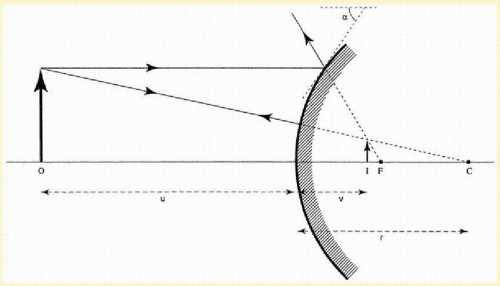
\includegraphics[scale=0.35]{ezgif.com-gif-maker (3).jpg}
    \caption{Optics of Keratometer}
    \label{fig:optics of keratometer}
\end{figure}
\subsection{Types of Keratometers}
\begin{itemize}
\item Hand-held autokeratometer
\item Humphrey autokeratometer
\item Bausch and Lomb	type keratometer
\item Javal-Schiotz keratometer	
\end{itemize}
\subsubsection{Bausch and Lomb principles}
The Bausch and Lomb Keratometer is a one position keratometer that gives readings in dioptric form. It differs from the Javal-Schiotz in that object size is fixed, image size is the manipulable variable. The reflected rays are passed through a Scheiner disc with 4 apertures – As there are two prisms, each aligned perpendicular to the other, the major and minor axis powers can be measured independently without adjusting the orientation of the instrument.
\subsubsection{Javal-Schiotz Principles}
The Javal-Schiotz keratometer is a two position instrument which uses a fixed image and doubling size and adjustable object size to determine the radius of curvature of the reflective surface. It uses two self illuminated mires (the object), one a red square, the other a green staircase design, which are held on a circumferential track in order to maintain a fixed distance from the eye. In order to get repeatable, accurate measurements, it is important that the instrument stays focused. It uses the Scheiner principle, common in autofocus devices, in which the converging reflected rays coming towards the eyepiece are viewed through (at least) two separate symmetrical apertures.
\begin{figure} [h]
    \centering
    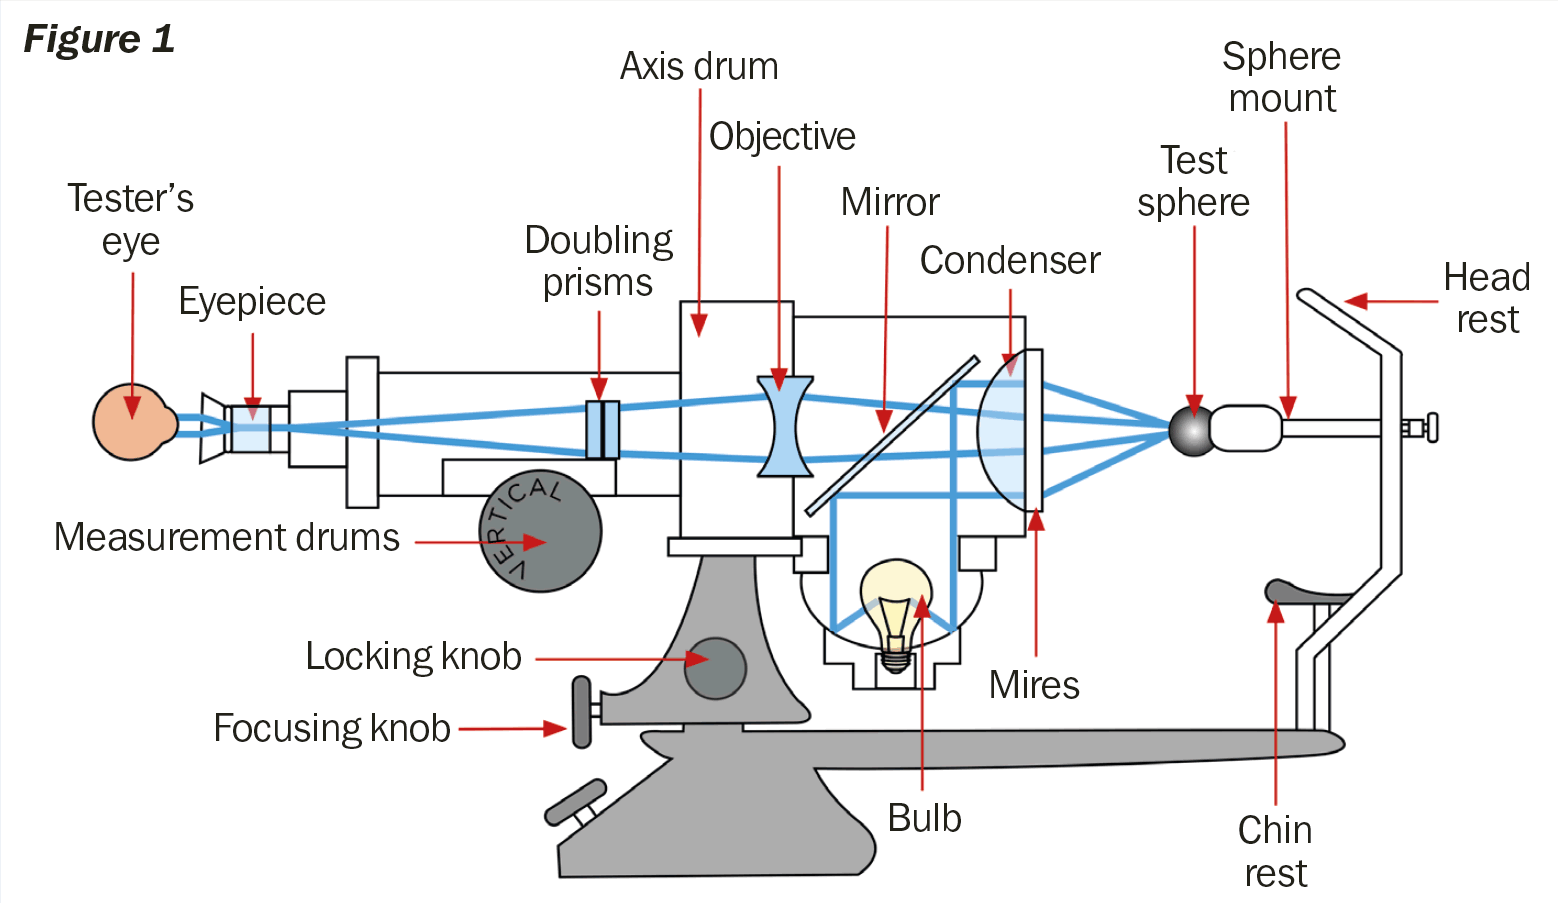
\includegraphics[scale=0.2]{figure12.png}
    \caption{Working of Keratometer}
    \label{fig:keratometer working}
\end{figure}
\subsection{Advantages of keratometer}
\begin{itemize}
\item Easy to use	
\item Inexpensive
\item Relatively accurate
\item Reproducible
\end{itemize}
\subsection{Limitations of keratometer}
\begin{itemize}
\item Assumption	that cornea	is	symmetrically spherical	or spherocylindrical
\item Measures small area	of	the	central	cornea	(3-4mm	diameter)
\item  Less accurate measuring irregular surfaces: very flat or steep cornea,	irregular	astigmatism
\item Does not quantify irregular astigmatism
\item One-position instruments assume	regular	astigmatism
\item Approximate	focal point and	refractive	index used in calculation
\item  The use of	paraxial optics	to calculate surface power
\item Limitations	in	detecting peripheral or	posterior keratoconus
\end{itemize}
\section{Laboratory safety cabinets(Biosafety Cabinets)}
Biosafety Cabinets (BSCs) are enclosed workspaces with a ventilated hood that is designed to contain pathogenic microorganisms during microbiological processes.
\begin{itemize}
\item The primary purpose of biosafety cabinets is to protect the laboratory personnel and the environment from the pathogenic microorganism as aerosols might be formed during the processing of such microorganisms.
\end{itemize}
\begin{itemize}
\item Biosafety cabinets are only used for certain risk group organisms and for processes that might result in aerosol formation.
\item These cabinets are provided with HEPA-filters that decontaminate the air moving out of the cabinet.
\item Biosafety cabinets might be confused with the laminar hood as both of these pieces of equipment work as enclosed workspaces. But, laminar hood only provides protection to the sample and not to the personnel and the environment, whereas biosafety cabinets protect all three.
\item The use of biosafety cabinets or other such physical containment is not required in the biosafety level 1, but depending on the risk assessment, some processes might require such containment.
\item BSCs are an essential part of biosafety as they minimize the formation of aerosol, protecting the environment, the pathogen, and the laboratory personnel.
\item Besides, most BSCs also function to sterilize biological materials that are kept inside the cabinets.
\end{itemize}
\subsection{Biosafety Cabinet Classes}
Biosafety cabinets are classified into three classes by the U.S. Centers for Disease Control and Prevention (CDC), each with specific performance characteristics and applications.
\begin{itemize}
\item Class I and II Biosafety cabinets are used for Biosafety levels I and II but, when used correctly in conjunction with useful microbiological techniques, these provide an effective containment system for safe manipulation of moderate and high-risk microorganisms.
\item Class III BSCs are most suitable for work with hazardous agents that require Biosafety Level 3 or 4.
\end{itemize}
\begin{figure} [h]
    \centering
    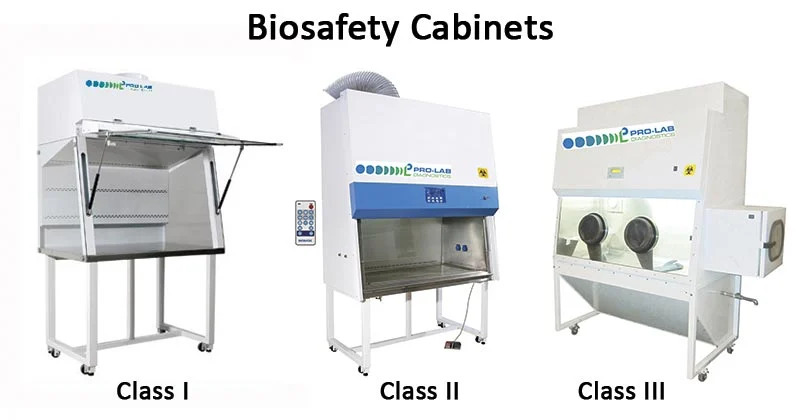
\includegraphics[scale=0.6,center]{ezgif.com-gif-maker (4).jpg}
    \caption{Biosafety Cabinet Classes}
    \label{fig:biosafety cabinet classes}
\end{figure}
\subsubsection{Biosafety Cabinet Class I}
\begin{itemize}
\item Class I is the most basic biosafety cabinet that provides protection to the environment and the laboratory personnel.
\item It doesn’t, however, provide protection to the product as the unsterilized room air is drawn over the work surface.
\item Class I biosafety cabinets are typically used to either enclose specific equipment like centrifuges or for procedures like aerating cultures that might potentially generate aerosols.
\item Biosafety cabinets of this class are either ducted (connected to the building exhaust system) or unducted (recirculating filtered exhaust back into the laboratory).
\item In the Class I BSC, the room air is drawn in through the opening that also allows the entry of the operator’s arm during work.
\item The air inside the cabinet then takes in the aerosol particles that may have been generated and moves it away from the operator towards the HEPA filter.The air moving out of the cabinet is thus, sterilized via the HEPA filters before its discharge to the environment.In this way, the cabinets protect the operator and the environment from the aerosol but not the sample.
\end{itemize}
\subsubsection{Biosafety Cabinet Class II}
\begin{itemize}
\item BSC-Class II cabinets provide both kinds of protection (of the samples and the environment) since makeup air is also HEPA-filtered.
\item The principle of operation of Class II cabinets involves a fan mounted in the top of the cabinet that draws a curtain of sterile air over the workstation where the biological products are being handled.
\item The air then moves underneath the work station and back up to the top of the cabinet before passing through the HEPA filters.The exhaust that moves out of the facility consists of air being drawn into the front of the cabinet underneath the work surface.The air drawn in acts as a barrier against the potentially contaminated air coming back out to the operator.
\item Class II BSCs are further divided into five types depending on the exhaust system and the mechanism of work (recirculation of the exhaust air); \textbf{Type A1}, \textbf{Type A2}, \textbf{Type B1}, \textbf{Type B2}, and \textbf{Type C1}.
\end{itemize}
\subsubsection{Biosafety Cabinet Class III}
\begin{itemize}
\item Class III cabinets are leak-tight, totally enclosed but ventilated cabinets, where all air that either enters or leaves through the facility pass through a HEPA filter.
\item The cabinets are provided with rubber gloves that are attached to the system to be used during operations in the cabinet. This is why these cabinets are also termed ‘glove boxes’.
\item The cabinet even has a transfer chamber that facilitates the sterilization of materials before they leave the glove box.Even though the gloves restrict the hand movement of the operator inside the cabinet, it prevents direct contact between the operator and the samples.The exhaust air is treated with double HEPA filters or HEPA filters in combination with incineration.
\item These cabinets can be used for all four Biosafety levels (1, 2, 3, and 4). But these are the most important for the manipulation of biological materials in the Biosafety level 4.
\item These cabinets are mostly custom-built for specific laboratories with lab equipment built inside the chamber.
\item All of these structural and design features provide maximum protection to the operator, the environment, and the sample against the high-risk group 4 pathogenic organisms.
\end{itemize}
















\end{document}
